% Author: PokMan Ho
% Script: res.tex
% Desc: MRes thesis result section
% Input: none
% Output: none
% Arguments: 0
% Date: Jan 2020

\documentclass[../thesis.tex]{subfiles} %% use packages & commands as this main file

\begin{document}
\section{Result}
%% text on all result -> all graphs
From Table \ref{tab:eqm}, P-only systems (eqm 3) could not give a biologically meaningful result for ``no harvest" setting under the current set of model assumptions.  Hence comparisons between with/without harvest were only done for P+B systems (eqm 4).  Comparing with/without carbon harvest in P+B systems (Fig.\ref{fig:wilcox}), the effort was statistically higher than ``no harvest" scenario only when the harvest rate was larger than 8/day.  Hence the closest significant sampled harvest rate with ``harvest" $>$ ``no harvest" was 9/day (W=57407, p=0.011).  However out of 1100 samples drew via LHS, about 90\% (n=991, median = -0.0016 (4dp)) feasible scenarios for ``no harvest" setting but only 12\% (n=134, median = 0.5670 (4dp)) for $x=9$/day.  On the other hand, P+B systems with harvest was statistically higher than their P-only counterparts for harvest rates higher than 1/day (Fig.\ref{fig:wilcox}).  At the closest significant sampled harvest rate with P+B $>$ P-only systems (2/day; W=129849, p$\ll$0.01), all (n=1100, median = -1.1334 (4dp)) scenarios were feasible for P-only system while only 25\% (n=275, median = -0.5379 (4dp)) for the P+B setting.

Effect of biological parameters on the model system (Eq.\ref{eq:ode}) was similar, hence the minimal significant P+B $>$ P-only system (i.e. $x=2$/day) was selected for discussion.  P+B systems with significant beneficial yield over ``no harvest" setting was bearing too few data for demonstration purposes due to much restricted feasible ranges on all biological parameters.  Total carbon stored in the system for P+B was always higher than that of P-only (Fig.\ref{fig:v2}).  Within the parameter ranges, low phytoplankton growth rate (min feasible $\gP$ = 0.3472/day (4dp)) and high non-respired carbon fraction for bacterial decomposer (max feasible $\eBR$ = 0.9129 (4dp)) could crash the respective systems.  Hence no such high efficient bacteria could be considered; only a P-only scenario could be applied for low growth rate phytoplanktons.  Within feasible parameter ranges, biological parameters affect their systems differently.  Increase in $\ePR$ would not alter much the total carbon in P+B systems but brought an increase for P-only systems.  Yield for P-only systems also rose faster than that of P+B and at high $\ePR$ scenarios P+B and P-only systems were largely similar

\begin{figure}[H]
    \centering
    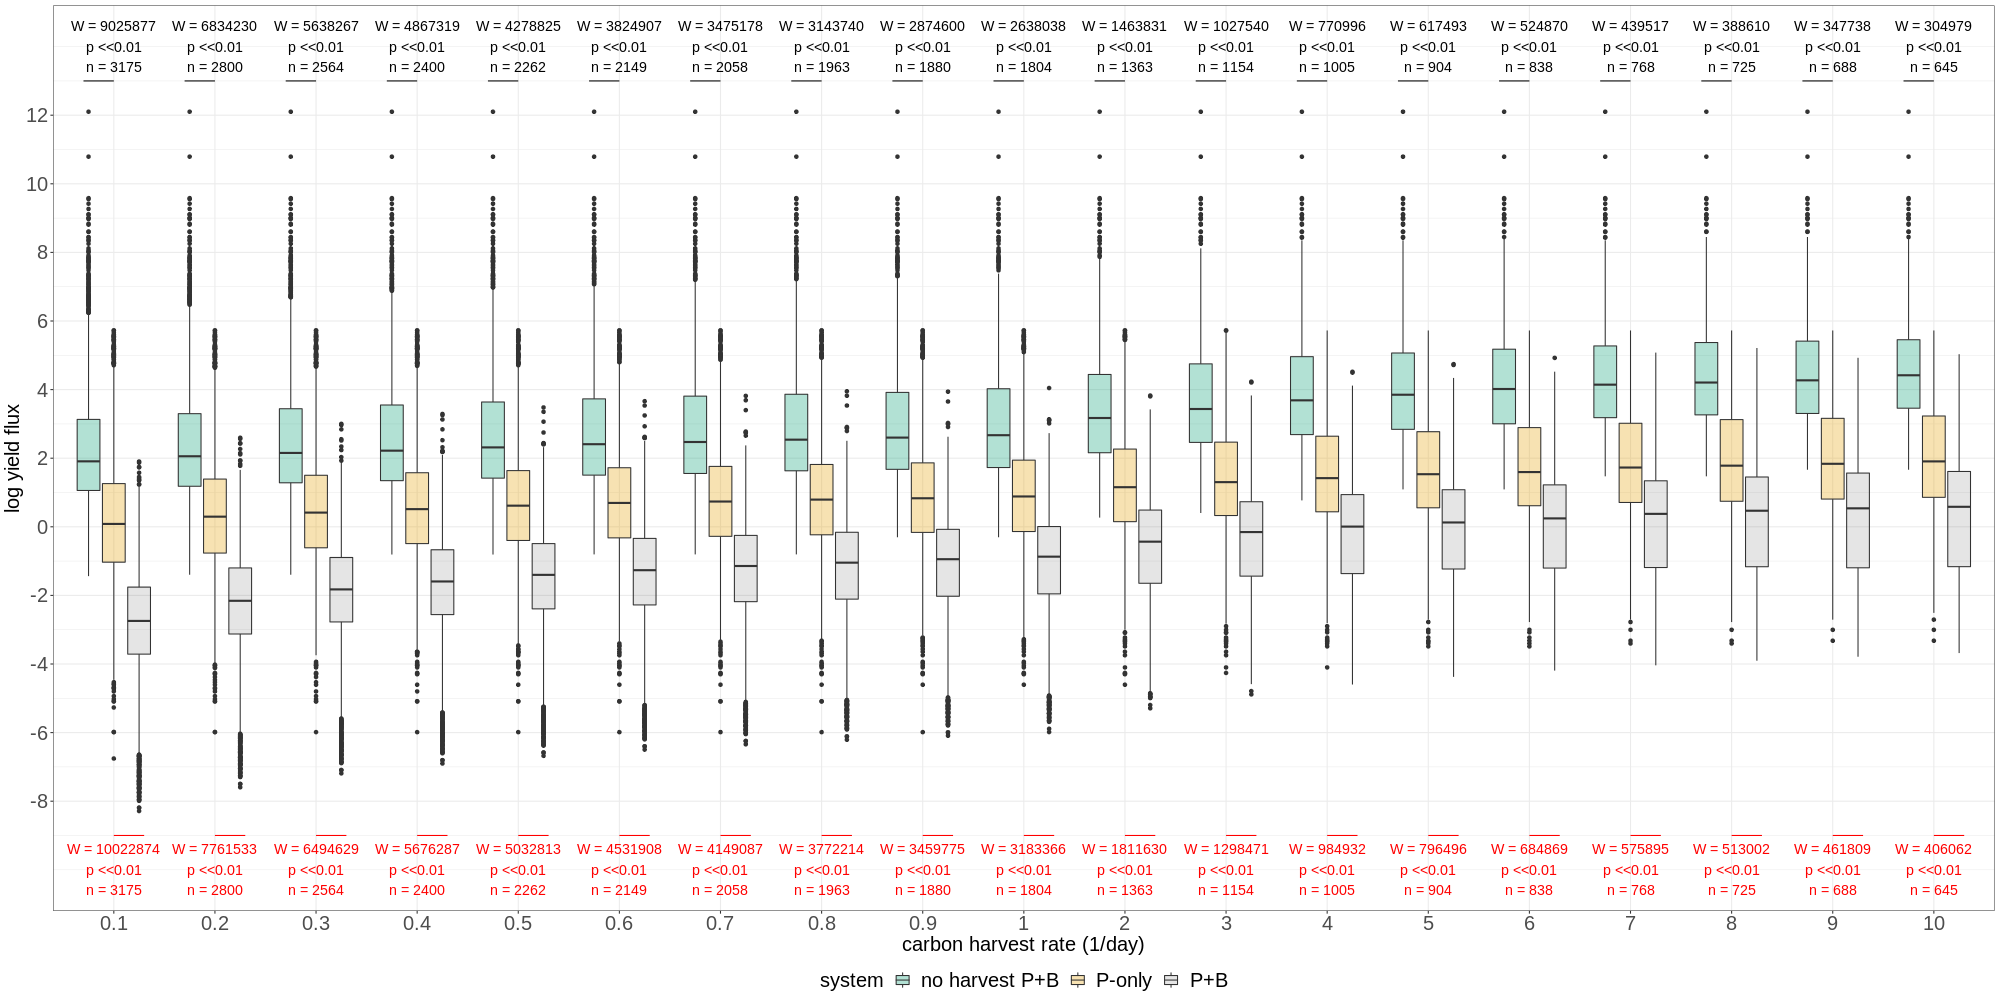
\includegraphics[width=\linewidth]{../result/Wilcox.png}
    \caption[Wilcox test summary]{Line graph showing Wilcox signed rank test (W-test) result (solid line) and respective p-values (dashed line) between P-only and P+B systems on ``log total carbon" and ``log yield flux" perspectives.  {\scriptsize The graph is based on the analytical simulations of the parameter hyperspace from LHS method.  Samples were divided into categories by carbon removal rate.  W-test was carried out between eqm 3 (P-only) and 4 (P+B) comparing the ranked mean distribution differences.}}
    \label{fig:wilcox}
\end{figure}

\begin{figure}[H]
    \centering
    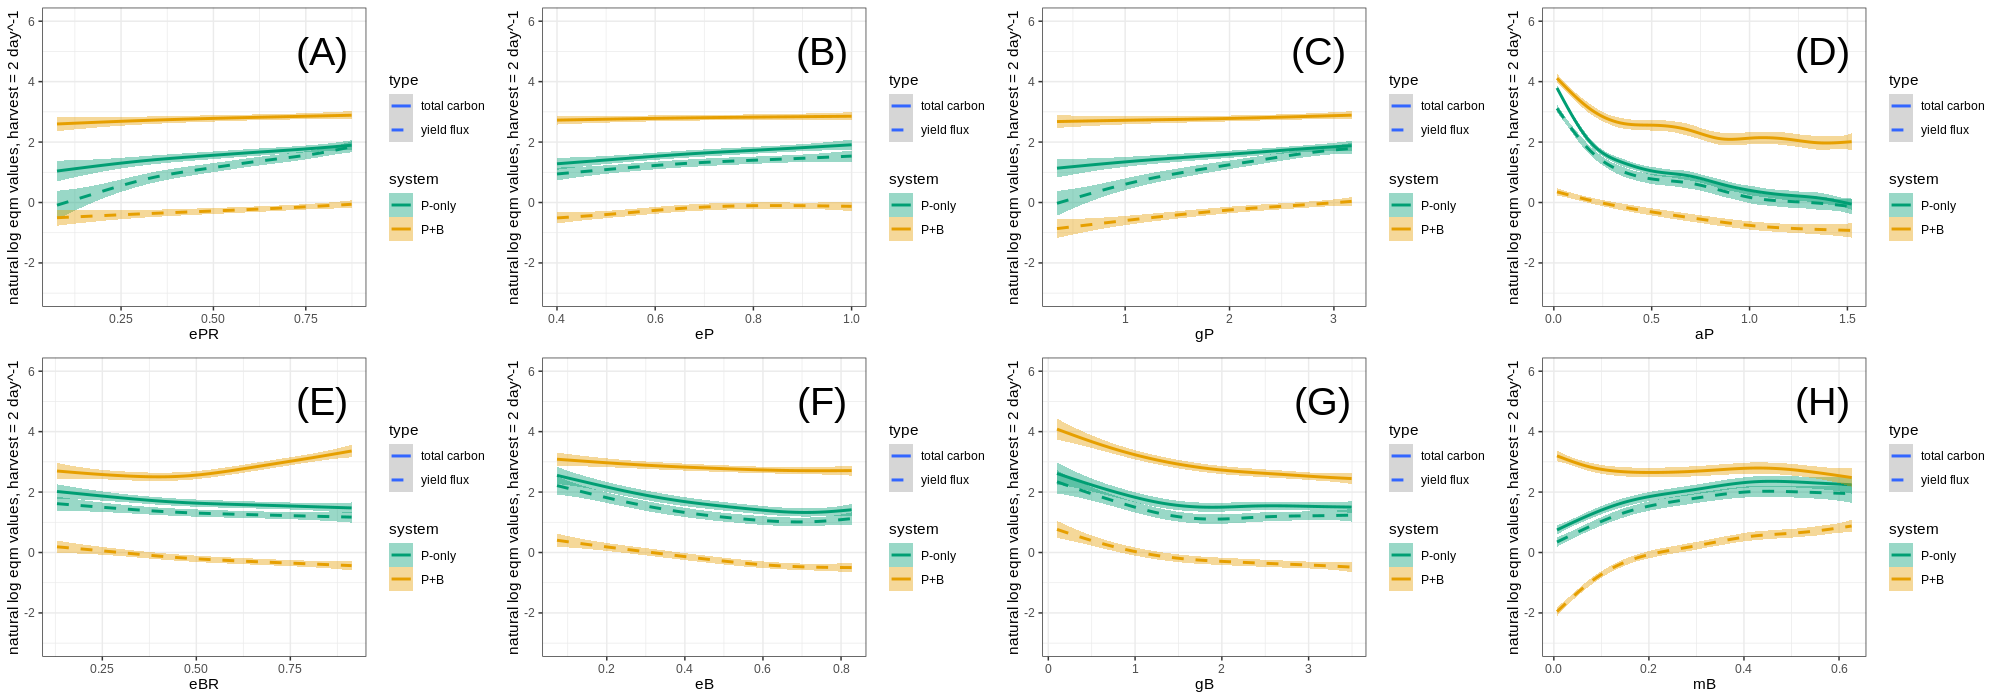
\includegraphics[width=\linewidth]{../result/var_20.png}
    \caption[95\% distribution for $x=2day^{-1}$]{Line graphs showing 95\% confidence interval for ``log total carbon" (solid line) and ``log yield flux" (dash line) based on respective parameter ranges when removal rate = 2$day^{-1}$.  {\scriptsize hi}}
    \label{fig:v2}
\end{figure}

\end{document}
